\section{Introduction}

\begin{figure}
	\centering
	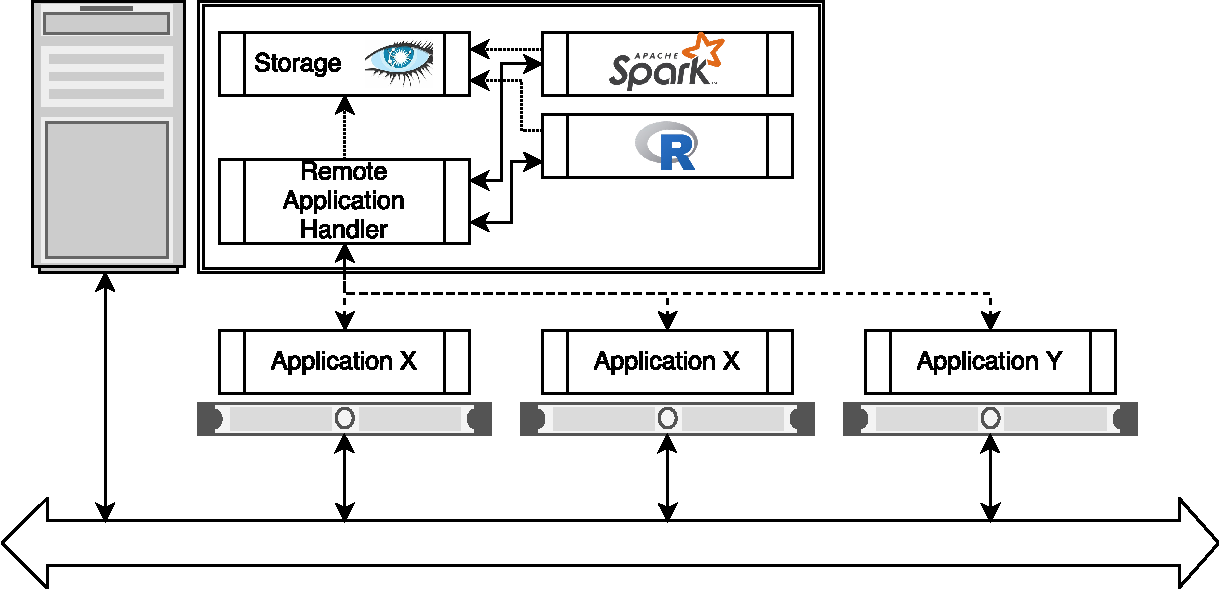
\includegraphics[scale=0.5]{overall_architecture}
	\caption{Overall architecture of the AGORA application handler.}
	\label{fig:architecture}
\end{figure}


The main goal of AGORA framework is to perform an online distributed Design Space Exploration.
The key concept is that on one hand we have the AGORA remote application handler that orchestrate the task; on the other hand, we have several instances of the application that explores the required configurations.

\prettyref{fig:architecture} shows the overall structure of the framework.
In particular, all the instances of the application executes on production nodes, for examples computing nodes of an HPC center, while the AGORA remote application handler runs in a dedicated server.
The communications between instances of application and the remote handler leverage the lightweight MQTT protocol, using the publish-subscribe pattern.
From a logical point of view, the remote application handler acts as a server, while the instances of application act as clients.

The typical workflow starts when the first instance of an unknown application begins to execute and notify its existence to the server.
The latter will ask to an application instance information about the application itself (e.g. the list of metrics of interest or the Design of Experiments required) and computes the set of configurations to explore.
At this point the server dispatch to clients the required configuration and it expects the observed performance of the application.
Once we have explored all the required configurations, it computes the application knowledge to broadcast to the clients.
In this way, all the instances of the application might start to leverage these information to automatically tune themselves.

The implementation of the agora application handler is designed to scale and to handle crash of clients.
In particular, the agora application handler uses a threadpool to process incoming message from clients, which might be instances of different applications.
It leverage Apache Cassandra\footnote{homepage: \url{http://cassandra.apache.org}} to store information about clients and uses a flexible plugin system to build the model of a metric of interest, starting from the observations.

The remainder of the manual is structured as follows: at first we describe in more details the remote application handler, then we discuss how the local application handler interacts with mARGOt.
The integration process is totally hidden by using the high-level interface mARGOt heel.
Please, refer to the mARGOt heel user guide for further details.
The last section of the document explain how to start the AGORA remote application handler.